%! TeX program = lualatex
\documentclass[main]{subfiles}

\begin{document}

\title[AutoML: BO]{Bayesian Optimization}
\subtitle{The Big Picture}
\author[Bernd Bischl]{Bernd Bischl}
\date{}

\titlebackground*{images/AutoML_HPO_2_2}

%\institute{}
%\date{}

    \maketitle


\begin{frame}[c]{Why Do We Need Bayesian Optimization?}

Many optimization problems in AutoML share three features:
\begin{itemize}
    \item The objective function is a \textbf{black box} -- no analytic form, no gradients
    \item Each evaluation is \textbf{expensive} -- training or resampling an ML model on a dataset can take minutes, hours, or days
    \item Evaluations are often \textbf{noisy} -- due to stochastic training, resampling, or measurement noise
\end{itemize}
\vspace{0.3cm}
\begin{center}
\textbf{Classic optimization methods do not fit well here}
\end{center}
\end{frame}

%----------------------------------------------------------------------

\begin{frame}{HPO Is a Black-Box Optimization Problem}
\begin{itemize}
    \item Finding a good hyperparameter configuration $\conf^\ast$ means solving
    $$\conf^\ast \in \argmin_{\conf \in \pcs} \cost(\conf)$$
    with
    $$\cost(\conf) = \riskg(\mathcal{I}(\datasettrain, \conf) \mid \datasetval)$$
    
    \item The mapping $\conf \mapsto \riskg(\dots)$ is exactly a black box:
    \begin{itemize}
        \item No closed-form expression
        \item Evaluation requires training / resampling a model
        \item Mixed / hierarchical search space 
    \end{itemize}
    \item $\riskg$ notation here is simplified to the use of a single validation set,
    in practice $\riskg$ might be a resampled performance, e.g. by using CV
    \item Same structure shows up beyond HPO: neural architecture search, pipeline construction, engineering design, scientific experiments\ldots
\end{itemize}
\end{frame}

%----------------------------------------------------------------------

\begin{frame}{ML Pipelines Can Also Be Configured}
\begin{itemize}
    \item A full ML \textbf{pipeline} chains preprocessing, feature engineering, learner, and post-processing
    \item Let $\conf$ encode \emph{all} pipeline choices, not just HPs of a single learner:
    \begin{itemize}
        \item Which imputation / scaling / encoding step
        \item Which feature selection or dimensionality reduction
        \item Which learner (e.g., random forest vs.\ SVM vs.\ gradient boosting)
        \item The hyperparameters of \emph{each} active component
    \end{itemize}
    \item The search space $\pcs$ becomes \textbf{hierarchical / conditional}:
    some hyperparameters are only active if a specific component was chosen
    \item The objective $\cost(\conf)$ is still a black box --\\
    BO can optimize over this combined pipeline + HP space
\end{itemize}
\end{frame}

%----------------------------------------------------------------------

\begin{frame}{Why Not Manual Tuning?}
\begin{itemize}
    \item Relies on expert intuition about the learner and the dataset
    \item Very inefficient and not automated
    \item Poorly reproducible -- choices are hard to document and communicate
    \item Prone to bias: \\
    humans revisit familiar settings and miss unusual but good regions
\end{itemize}
\vspace{0.3cm}
\begin{center}
\textbf{We want a systematic, adaptive, and reproducible alternative.}
\end{center}
\end{frame}

%----------------------------------------------------------------------

\begin{frame}{Why Not Just Grid or Random Search?}
\begin{columns}
    \column{.55\textwidth}
    \begin{itemize}
        \item Simple, parallelizable, hard to beat as a baseline
        \item But: they are \textbf{non-adaptive}
        \begin{itemize}
            \item Every configuration is sampled independently of previous results
            \item Budget is wasted on obviously unpromising regions
        \end{itemize}
        \item Scaling is poor in higher-dimensional search spaces
        \item For expensive objectives we want an optimizer that \textbf{learns from its own evaluations}
    \end{itemize}
    \column{.4\textwidth}
    \begin{center}
        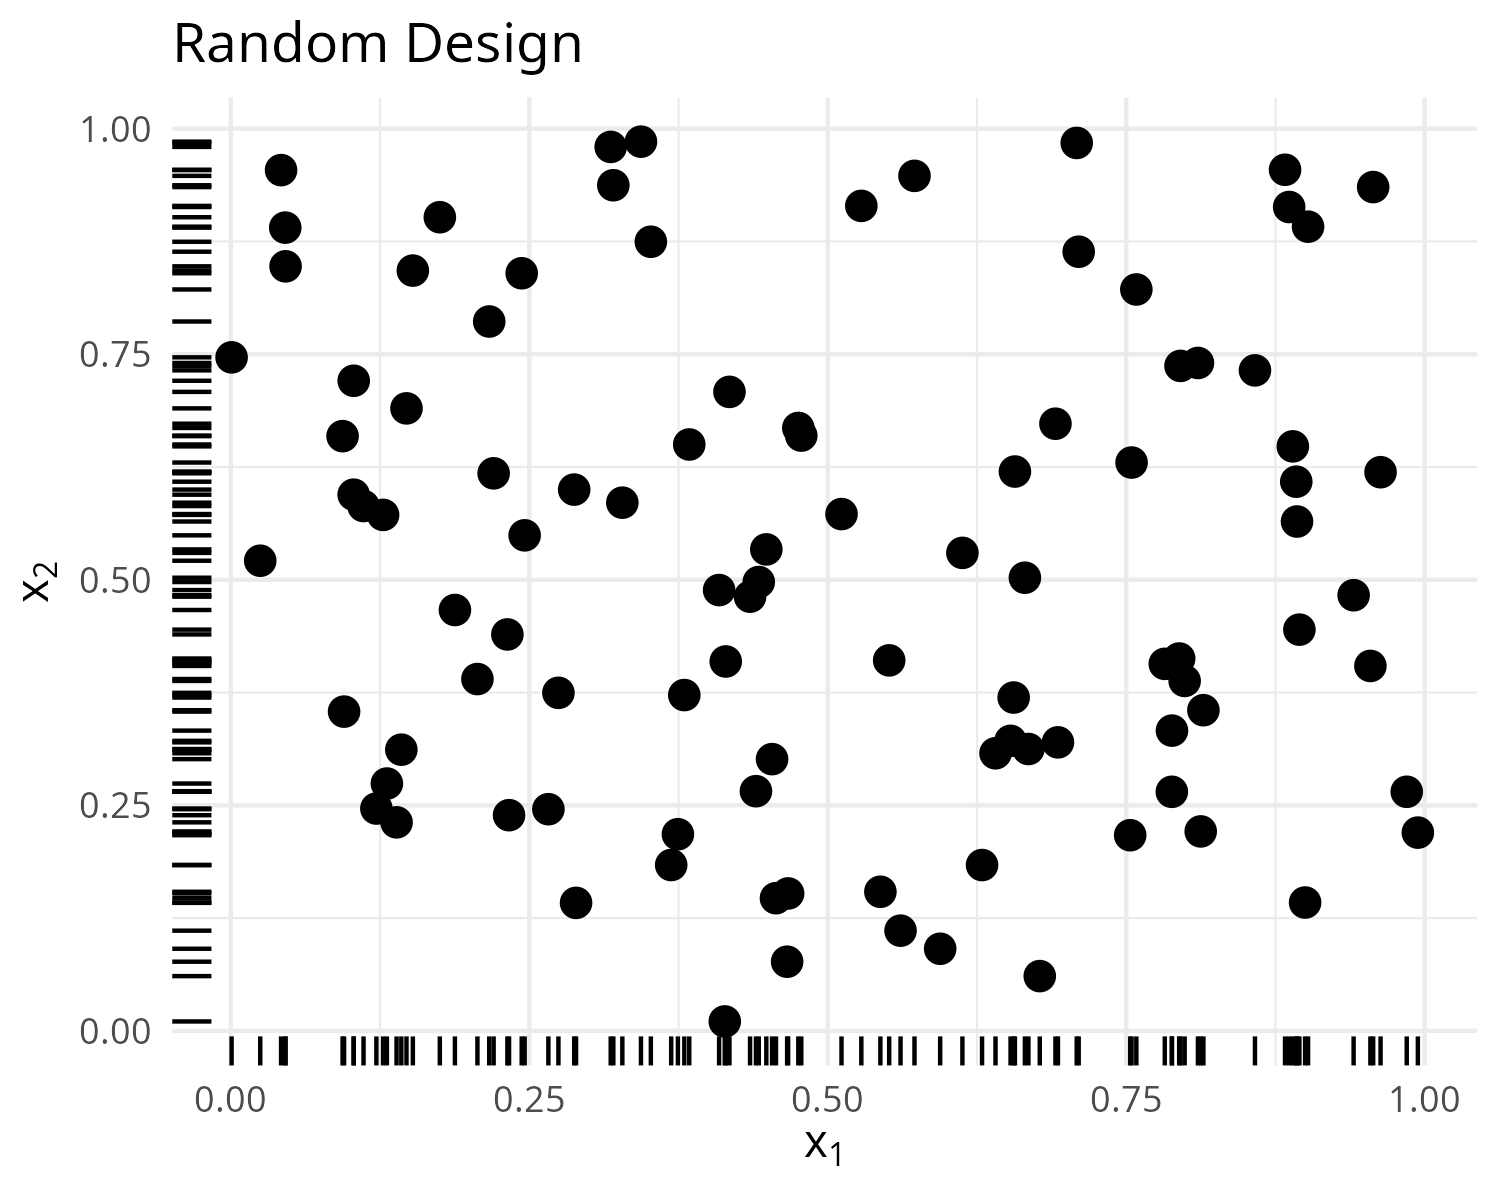
\includegraphics[width=\textwidth]{images/black_box_0.png}\\
        \footnotesize Random search on a 2D landscape.
    \end{center}
\end{columns}
\end{frame}

%----------------------------------------------------------------------

\begin{frame}{The Core Idea of Bayesian Optimization}
\begin{itemize}
    \item Fit a cheap \textbf{surrogate model} $\surro$ to the observations collected so far
    \item Use the surrogate to form an \textbf{acquisition function} that trades off
    \begin{itemize}
        \item \textbf{Exploitation:} sample where $\surro$ predicts good values
        \item \textbf{Exploration:} sample where $\surro$ is uncertain
    \end{itemize}
    \item Evaluate the true objective only at the most \textbf{informative} point, update the surrogate, repeat
\end{itemize}
\vspace{0.3cm}
\begin{center}
\textbf{Sequential, model-based, sample-efficient} -- designed for exactly the setting where each evaluation is precious.
\end{center}
\end{frame}

%----------------------------------------------------------------------

\begin{frame}{Why Care Specifically in AutoML?}
\begin{itemize}
    \item BO is the \textbf{backbone} of many modern AutoML systems (e.g., SMAC, Spearmint, BoTorch, Optuna)
    \item It is typically much more \textbf{sample-efficient} than random or evolutionary search on HPO benchmarks
    \item It provides a principled way to handle
    \begin{itemize}
        \item Noisy evaluations
        \item Multiple objectives (accuracy vs.\ runtime, vs.\ fairness, \ldots)
        \item Mixed / hierarchical configuration spaces
    \end{itemize}
    \item Many advanced HPO ideas (multi-fidelity, warmstarting, priors) build directly on top of BO
\end{itemize}
\end{frame}

%----------------------------------------------------------------------

\begin{frame}{Guiding Questions for This Chapter}
\begin{itemize}
    \item What makes an optimization problem a ``black-box'' problem?
    \item What does the basic BO loop look like?
    \item How do we quantify uncertainty with a surrogate model?
    \item How do acquisition functions (LCB, PI, EI) balance exploration and exploitation?
    \item Which surrogate models are useful in practice (GPs, random forests)?
    \item How do we handle noise and multiple objectives?
    \item Which practical choices matter when implementing or using BO?
\end{itemize}
\end{frame}

%----------------------------------------------------------------------

\begin{frame}{Summary}
\begin{enumerate}
    \item HPO and many AutoML tasks are expensive, noisy, black-box optimization problems
    \item Grid and random search are non-adaptive and waste evaluations
    \item Bayesian optimization uses a surrogate model and an acquisition function to pick \emph{informative} points, making it sample-efficient
    \item BO is a key building block for modern AutoML systems
\end{enumerate}
\vspace{0.3cm}
$\leadsto$ The rest of this chapter develops the BO loop, surrogate models, and acquisition functions in detail.
\end{frame}

\end{document}
